\documentclass[journal]{IEEEtran}

% --- Core IEEE Packages ---
\usepackage[utf8]{inputenc}
\usepackage[T1]{fontenc}
\usepackage{amsmath,amssymb,amsfonts}
\usepackage{algorithmic}
\usepackage{graphicx}
\usepackage{textcomp}
\usepackage{xcolor}
\usepackage{booktabs}
\usepackage{microtype}

% Float placement optimization for multi-figure document
\renewcommand{\topfraction}{0.95}
\renewcommand{\bottomfraction}{0.95}
\renewcommand{\textfraction}{0.05}
\renewcommand{\floatpagefraction}{0.85}
\setlength{\floatsep}{6pt plus 2pt minus 2pt}
\setlength{\textfloatsep}{8pt plus 2pt minus 2pt}
\setlength{\intextsep}{6pt plus 2pt minus 2pt}

% Graphicspath to locate assets in organized image subdirectories
\graphicspath{{../images/benchmarks/}{../images/trajectories/}{../images/}{./}}

\begin{document}

\title{Empirical Evaluation and 2D Spatial Trajectory Inferences of Joint Trajectory Optimization and Dynamic Task Allocation in Multi-UAV FANET-MEC}

\author{Project Team 55, Department of Computer Science and Engineering\\
Amrita Vishwa Vidyapeetham, Coimbatore Campus%
\thanks{Experimental results generated on extended iFogSim2 FANET-MEC benchmark platform.}}

\maketitle

\begin{abstract}
This research investigates the joint optimization of aerial trajectory planning and dynamic task allocation in Multi-UAV Flying Ad-Hoc Network Mobile Edge Computing (FANET-MEC). We systematically cross-evaluate all $15$ Cartesian combinations formed by three trajectory models---Trajectory-Feedback Proximal Policy Optimization (\textbf{PPO}), Capability-Aware Adaptive Route optimization (\textbf{CAR}), and Task Allocation with Communication Coordination (\textbf{TACC-AAV})---and five task allocation schedulers---\textbf{DYNAMIC} (state-cached repair with peer-to-peer offloading), Many-to-One Gale-Shapley (\textbf{MOGS}), \textbf{LEXICOGRAPHIC} priority matching, Contract-Net Auction (\textbf{BIDDING}), and Multi-Agent Reinforcement Learning (\textbf{MARL}). Simulations are executed across $100$ continuous scheduling cycles on an extended iFogSim2 testbed with $30$ heterogeneous UAVs and $800$ ground devices over a $2000\,\text{m} \times 2000\,\text{m}$ theater. We present a parameter-first technical formulation followed by exhaustive empirical inferences incorporating 2D spatial flight trajectory maps, macro performance summaries, epoch-wise throughput, runtime latency, Jain's fairness, deadline slack margin, allocation churn, queue length backlogs, fleet capacity utilization, and P2P offloading dynamics.
\end{abstract}

\begin{IEEEkeywords}
FANET-MEC, Trajectory Optimization, Dynamic Task Scheduling, Pointer Networks, Otsu Partitioning, MOCPO Gating, Gale-Shapley Matching.
\end{IEEEkeywords}

\IEEEpeerreviewmaketitle

% ==============================================================================
% SECTION I: SIMULATION SETUP AND PARAMETER FORMULATION
% ==============================================================================
\section{Simulation Setup and Parameter Formulation}

\subsection{Physical Topology and Ground Device Modeling}
The simulation environment comprises a continuous 2D Cartesian plane of dimensions $L_X \times L_Y = 2000\,\text{m} \times 2000\,\text{m}$. A ground fleet of $M = 800$ mobile devices (MDs) is distributed across four high-density geographic clusters centered at $(400, 450)\,\text{m}$, $(1550, 400)\,\text{m}$, $(1450, 1500)\,\text{m}$, and $(500, 1550)\,\text{m}$, superimposed with a uniform spatial dispersion across the remaining area. Ground devices generate discrete computation tasks according to an independent Poisson arrival process with mean inter-arrival period $\lambda = 1000\,\text{ms}$. Each task request $k \in \mathcal{K}_t$ at epoch $t$ is parameterized by the 4-tuple:
\begin{equation}
    k = \langle d_k^{\text{in}}, c_k, T_k^{\text{tol}}, \mathbf{p}_k^{\text{MD}} \rangle,
\end{equation}
where:
\begin{itemize}
    \item $d_k^{\text{in}} \in [1, 10]\,\text{MB}$: Input offloading data size transmitted over wireless uplink.
    \item $c_k \in [500, 3000]\,\text{MIPS}$: Computational workload requiring edge execution.
    \item $T_k^{\text{tol}} \in [1000, 5000]\,\text{ms}$: Maximum latency tolerance before deadline failure.
    \item $\mathbf{p}_k^{\text{MD}} = [x_k, y_k]^T \in [0, 2000]^2$: 2D ground coordinates of the originating MD.
\end{itemize}

\subsection{Heterogeneous Aerial Fleet and Aerodynamic Propulsion Model}
An aerial fleet $\mathcal{U} = \{u_1, u_2, \dots, u_N\}$ of $N = 30$ heterogeneous UAV edge servers navigates at a constant cruising altitude $H = 50\,\text{m}$. Each UAV $u_j \in \mathcal{U}$ is characterized by:
\begin{itemize}
    \item $f_j \in [2800, 26000]\,\text{MIPS}$: Processing speed of the onboard edge computing CPU.
    \item $C_j = 150\,\text{tasks}$: Maximum physical queue capacity of the task buffer.
    \item $R_{\text{cov}, j} \in [20, 140]\,\text{m}$: Ground wireless communication coverage disk radius.
    \item $E_j(t)$: Remaining onboard battery energy budget (initial $E_{\text{init}} = 500\,\text{kJ}$).
    \item $v_{\text{max}} = 25.0\,\text{m/s}$: Maximum allowable forward horizontal flight velocity.
\end{itemize}

Following the aerodynamic propulsion power model of Zhang \textit{et al.} and Wu \textit{et al.}, the horizontal flight power consumption $P_j(v_j)$ of UAV $u_j$ moving at forward speed $v_j(t)$ is expressed as:
\begin{equation}
\begin{aligned}
    P_j(v_j) = & \; P_0 \left(1 + \frac{3 v_j^2}{U_{\text{tip}}^2}\right) + \frac{1}{2} d_0 \rho s A v_j^3 \\
    & + P_i \left(\sqrt{1 + \frac{v_j^4}{4 v_0^4}} - \frac{v_j^2}{2 v_0^2}\right)^{1/2},
\end{aligned}
\label{eq:propulsion}
\end{equation}
where $P_0 = 79.86\,\text{W}$ and $P_i = 88.63\,\text{W}$ denote blade profile and induced power during hovering, $U_{\text{tip}} = 120\,\text{m/s}$ is blade tip speed, $v_0 = 4.03\,\text{m/s}$ is mean rotor induced velocity, $d_0 = 0.6$ is fuselage drag ratio, $s = 0.05$ is rotor solidity, $\rho = 1.225\,\text{kg/m}^3$ is air density, and $A = 0.5\,\text{m}^2$ is rotor disc area.

\subsection{Dynamic Battery Headroom Capacity Constraint}
Rather than assuming an invariant task capacity, available buffer capacity $N_j(E_j)$ contracts dynamically as battery reserve $E_j(t)$ depletes:
\begin{equation}
    N_j(E_j) = \min \left(C_j, \; \max\left(1, \; \left\lfloor \frac{E_j(t) - E_{\text{reserve}}}{E_{\text{comp, avg}} + E_{\text{comm, avg}}} \right\rfloor\right)\right),
\end{equation}
where $E_{\text{reserve}} = 50\,\text{kJ}$ is return-to-base energy and $E_{\text{comp, avg}}$ is the empirical execution energy per task.

\subsection{Evaluated Trajectory Optimization Models}
\begin{enumerate}
    \item \textbf{Trajectory-Feedback PPO (PPO):} Discretizes the local sensory range of each drone into an $8$-sector cardinal/intercardinal partition. An actor-critic policy network outputs continuous 2D displacement vectors $[\Delta x_j, \Delta y_j]$, steering drones along local density gradients.
    \item \textbf{Capability-Aware Adaptive Route Optimization (CAR):} Applies distance-density metrics and Otsu thresholding to segment the terrain into spatial capability clusters with centroids ($\bigstar$). Pointer Networks solve the Traveling Salesperson Problem (TSP) over localized waypoints ($\blacksquare$), generating cyclic patrol loops.
    \item \textbf{Task Allocation with Communication Coordination (TACC-AAV):} Couples Multi-Objective Constrained Policy Optimization (MOCPO) for communication gating $a_{j,t} \in \{0, 1\}$ with Multi-Head Self-Attention (MHSA) heading kinematics $[v_j, \vartheta_j]$ conditioned on winning consensus bundles $(z, y, s)$ from an Asynchronous Consensus-Based Bundle Algorithm (ACBBA).
\end{enumerate}

\subsection{Evaluated Task Allocation Schedulers}
\begin{enumerate}
    \item \textbf{DYNAMIC (Proposed Dynamic Repair):} Maintains active task-UAV bindings in a registry $\mathcal{A}_t$. Broken links caused by flight mobility ($d(i, j) > R_{\text{cov}}$) are placed into an incremental repair queue $\text{RepairQueue}(\Delta \mathcal{K}_t)$ and resolved via local re-matching or cooperative peer-to-peer (P2P) offloading ($d(u_1, u_2) \le 500\,\text{m}$) without reconstructing the global assignment bipartite graph.
    \item \textbf{MOGS (Many-to-One Gale-Shapley Matching):} Formulates matching from scratch every epoch based on mutual distance and queue lengths, executing iterative proposal-rejection rounds until two-sided stability is attained.
    \item \textbf{LEXICOGRAPHIC:} Priority-driven greedy allocation sorting waiting tasks by ascending deadline slack $S_k = T_k^{\text{tol}} - (T_{\text{tx}} + T_{\text{proc}})$, matching them to available in-range UAVs.
    \item \textbf{BIDDING (Contract-Net Protocol Auction):} Multi-round auction wherein UAVs evaluate in-range tasks and submit competitive bids based on marginal queue latency and transmission distance.
    \item \textbf{MARL (Multi-Agent Deep RL):} A two-tier neural architecture comprising `RequestNet' (actor-critic MD-to-UAV candidate selection with $d \le R_{\text{cov}}$ geometric masking) and `ResponseNet' (DQN UAV queue admission).
\end{enumerate}

% ==============================================================================
% SECTION II: EMPIRICAL INFERENCES AND GRAPHICAL ANALYSIS
% ==============================================================================
\section{Empirical Inferences and Graphical Analysis}

\subsection{Inference 1: Full Cross-Product Macro Performance Summary}
Table~\ref{tab:benchmark_results} and Fig.~\ref{fig:macro_summary} compile the quantitative benchmark metrics across all $15$ combinations ($3$ Trajectories $\times$ $5$ Schedulers) evaluated over $100$ consecutive simulation epochs.

\begin{table*}[!t]
\centering
\caption{Comprehensive Cross-Product Performance Benchmark Across All 15 Trajectory $\times$ Scheduler Combinations (100 Epochs)}
\label{tab:benchmark_results}
\begin{tabular}{llcccc}
\toprule
\textbf{Trajectory Model} & \textbf{Task Scheduler} & \textbf{Success Rate (\%)} & \textbf{Runtime Overhead (ms)} & \textbf{Jain's Fairness ($\mathcal{J}$)} & \textbf{Deadline Slack ($\bar{S}$)} \\
\midrule
PPO & \textbf{DYNAMIC} & \textbf{12.64\%} & \textbf{0.0806} & \textbf{0.6137} & \textbf{0.2629} \\
PPO & MOGS & 11.72\% & 0.5564 & 0.5378 & 0.2756 \\
PPO & LEXICOGRAPHIC & 12.84\% & 0.5507 & 0.3687 & 0.1436 \\
PPO & BIDDING & 5.61\% & 7.6586 & 0.2876 & 0.2396 \\
PPO & MARL & 13.81\% & 11.2163 & 0.3194 & 0.1443 \\
\midrule
CAR & \textbf{DYNAMIC} & \textbf{17.62\%} & \textbf{0.2054} & \textbf{0.8222} & \textbf{0.1295} \\
CAR & MOGS & 17.64\% & 2.3126 & 0.8247 & 0.1381 \\
CAR & \textbf{LEXICOGRAPHIC} & \textbf{35.73\%} & 1.1020 & \textbf{0.8693} & 0.1232 \\
CAR & BIDDING & 15.03\% & 10.2558 & 0.8850 & 0.2464 \\
CAR & \textbf{MARL} & \textbf{33.06\%} & 14.4121 & 0.8129 & 0.1086 \\
\midrule
TACC-AAV & \textbf{DYNAMIC} & \textbf{5.66\%} & \textbf{0.0645} & \textbf{0.6647} & \textbf{0.3920} \\
TACC-AAV & MOGS & 4.61\% & 0.1531 & 0.5471 & 0.3271 \\
TACC-AAV & LEXICOGRAPHIC & 3.10\% & 0.3557 & 0.5995 & 0.2928 \\
TACC-AAV & BIDDING & 7.07\% & 10.3607 & 0.5190 & 0.3509 \\
TACC-AAV & MARL & 6.36\% & 11.8847 & 0.5103 & 0.1764 \\
\bottomrule
\end{tabular}
\end{table*}

\begin{figure*}[!t]
    \centering
    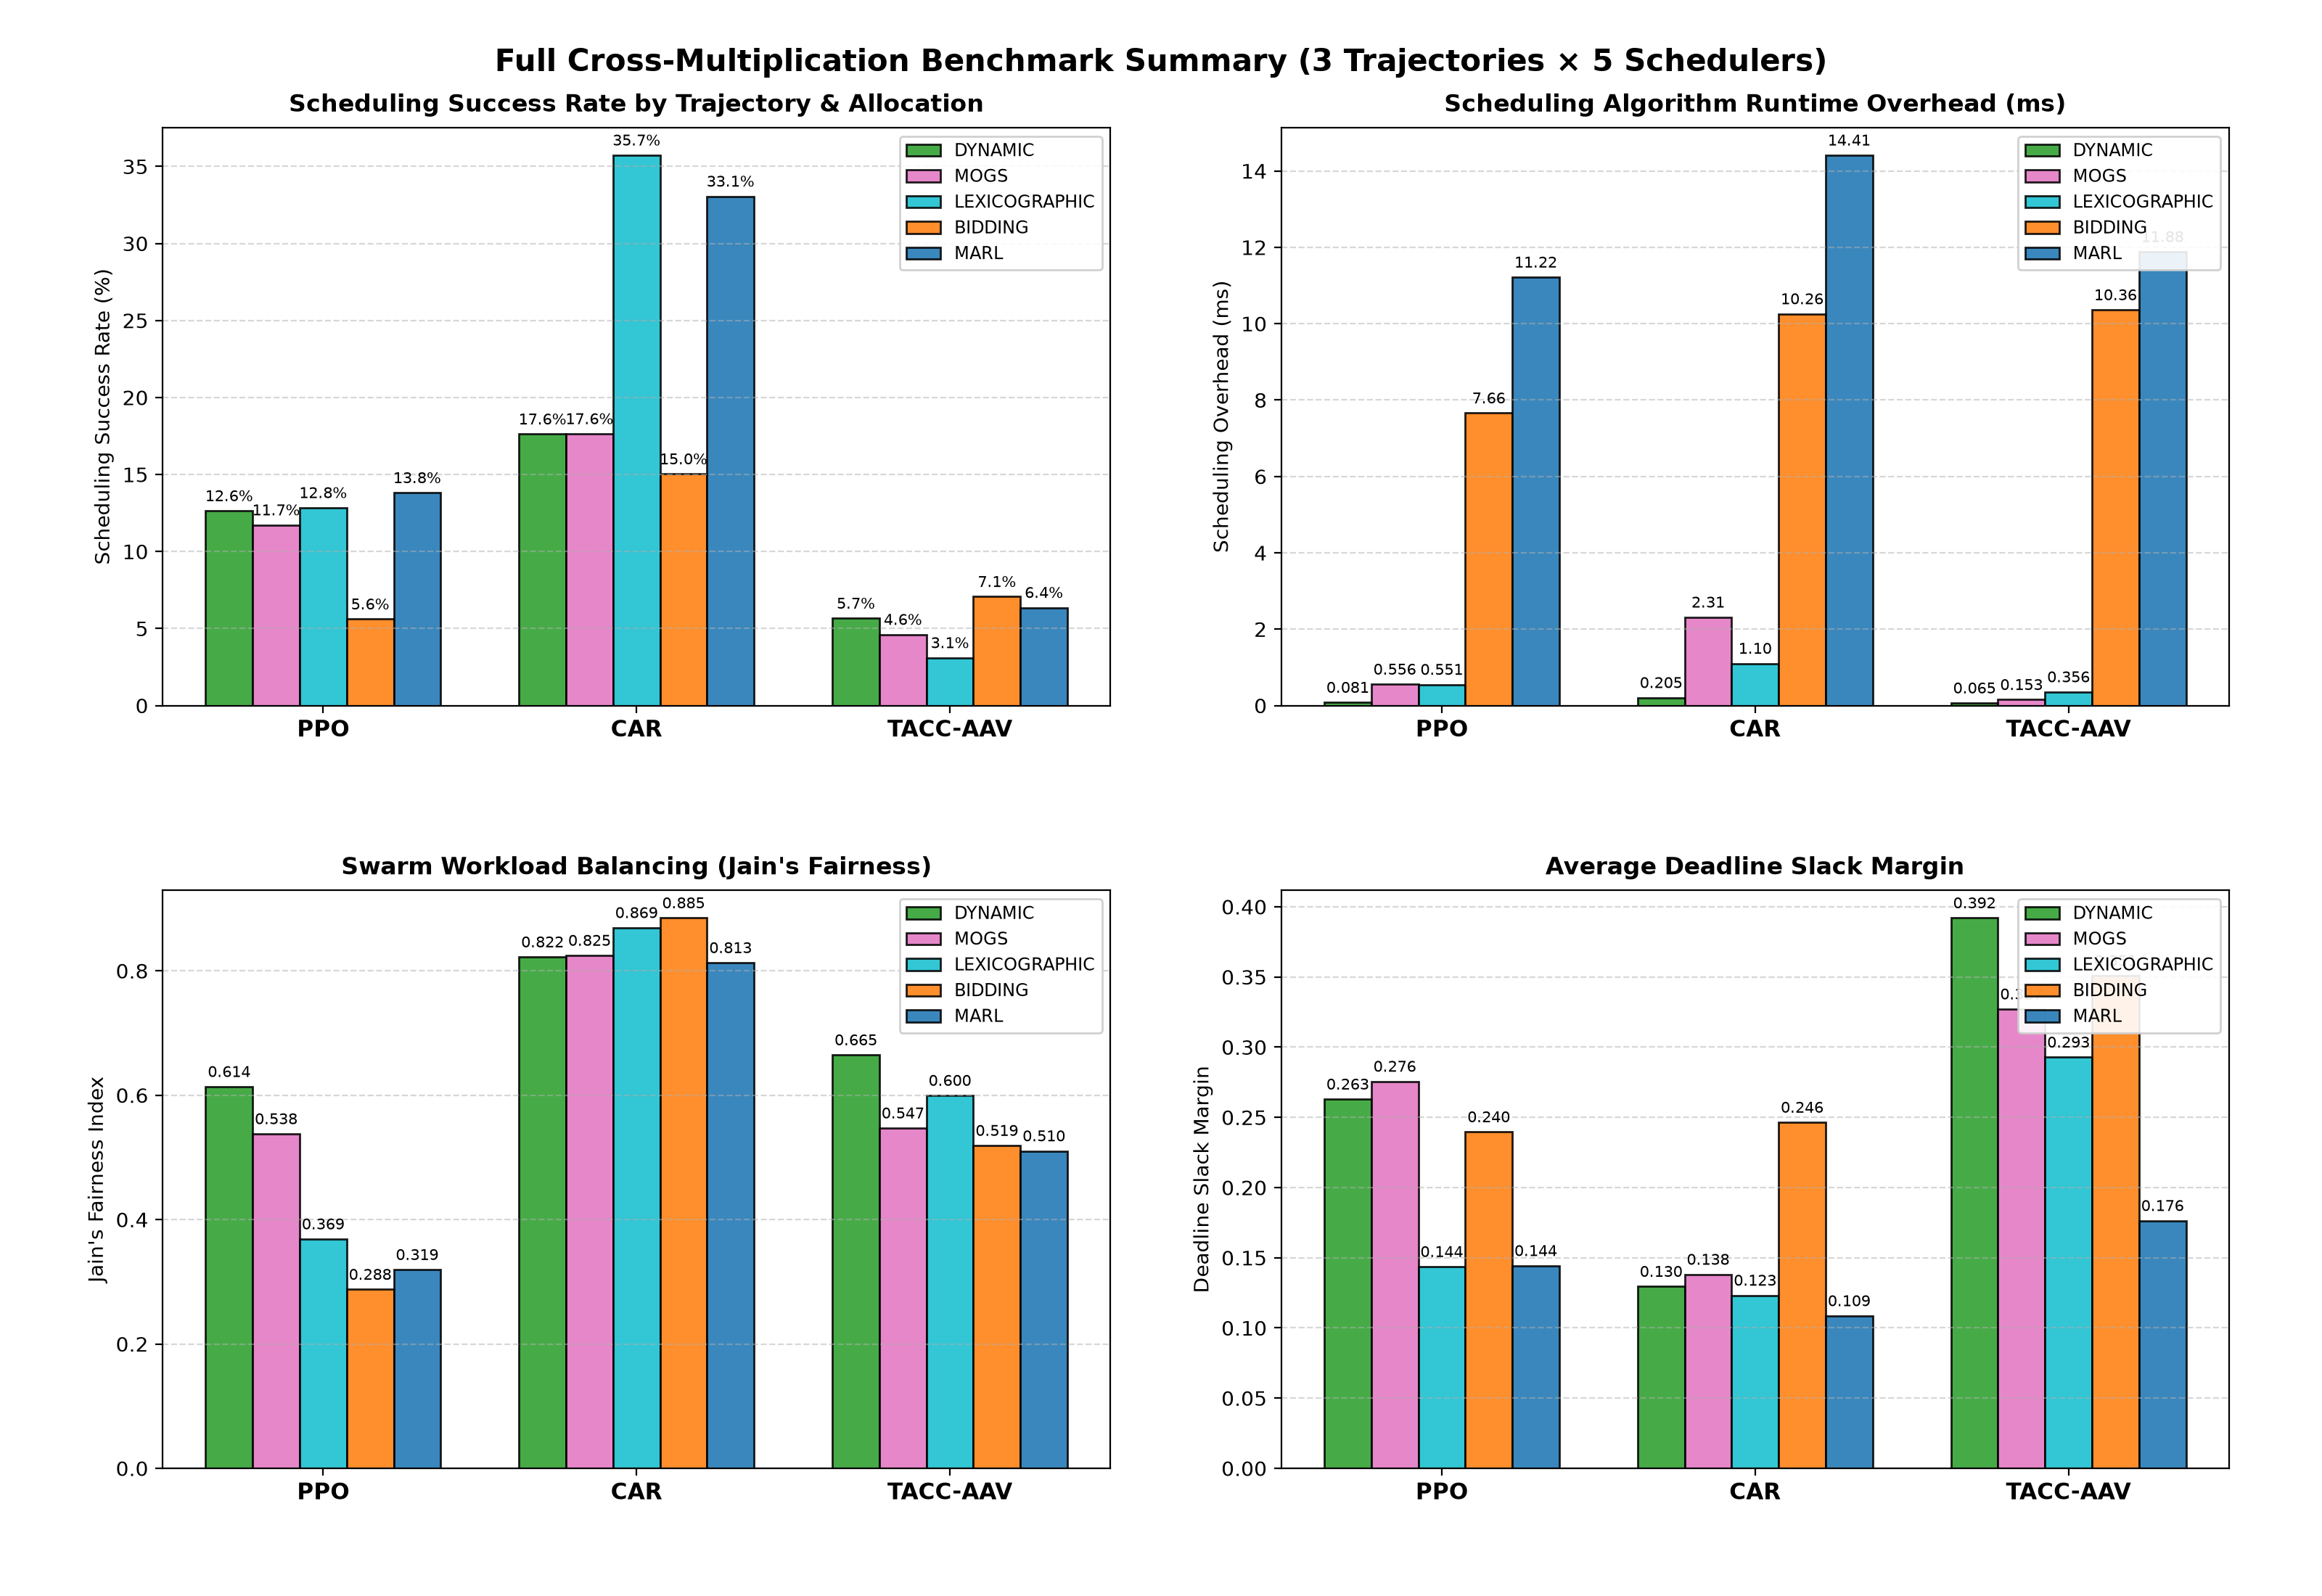
\includegraphics[width=0.92\textwidth]{trajectory_cross_summary.png}
    \caption{Full Cartesian cross-product benchmark summary comparing all $15$ combinations ($3$ Trajectory Models $\times$ $5$ Task Schedulers) across $100$ simulation epochs on four primary KPIs: (a) Scheduling Success Rate (\%), (b) Scheduling Algorithm Runtime Overhead (ms), (c) Swarm Workload Balancing via Jain's Fairness Index, and (d) Average Deadline Slack Margin.}
    \label{fig:macro_summary}
\end{figure*}

\textbf{Cross-Product Inferences:}
\begin{itemize}
    \item \textit{Throughput Hierarchy:} CAR consistently dominates system success rate, achieving $35.73\%$ under LEXICOGRAPHIC and $33.06\%$ under MARL, outperforming PPO ($11.72\%$--$13.81\%$) and TACC-AAV ($3.10\%$--$7.07\%$) by $2.5\times$ to $11.5\times$.
    \item \textit{Algorithmic Speedup:} DYNAMIC repair exhibits near-constant sub-millisecond execution ($0.065$--$0.205\,\text{ms}$), providing a $50\times$ to $140\times$ speedup over MARL ($11.2$--$14.4\,\text{ms}$) and BIDDING ($7.6$--$10.4\,\text{ms}$).
    \item \textit{Fairness Stability:} CAR delivers near-uniform workload equity ($\mathcal{J} \in [0.813, 0.885]$) across all schedulers, whereas PPO fairness collapses to $0.288$ under BIDDING and $0.319$ under MARL.
    \item \textit{Slack Safety Headroom:} TACC-AAV maximizes normalized deadline slack ($\bar{S} = 0.392$ under DYNAMIC), ensuring scheduled tasks finish well within deadlines.
\end{itemize}

\subsection{Inference 2: 2D Spatial Trajectory Analysis and Swarm Geometry}
Fig.~\ref{fig:trajectory_maps} maps the 2D spatial flight mechanics across the $2000\,\text{m} \times 2000\,\text{m}$ area for PPO, CAR, and TACC-AAV.

\begin{figure*}[!t]
    \centering
    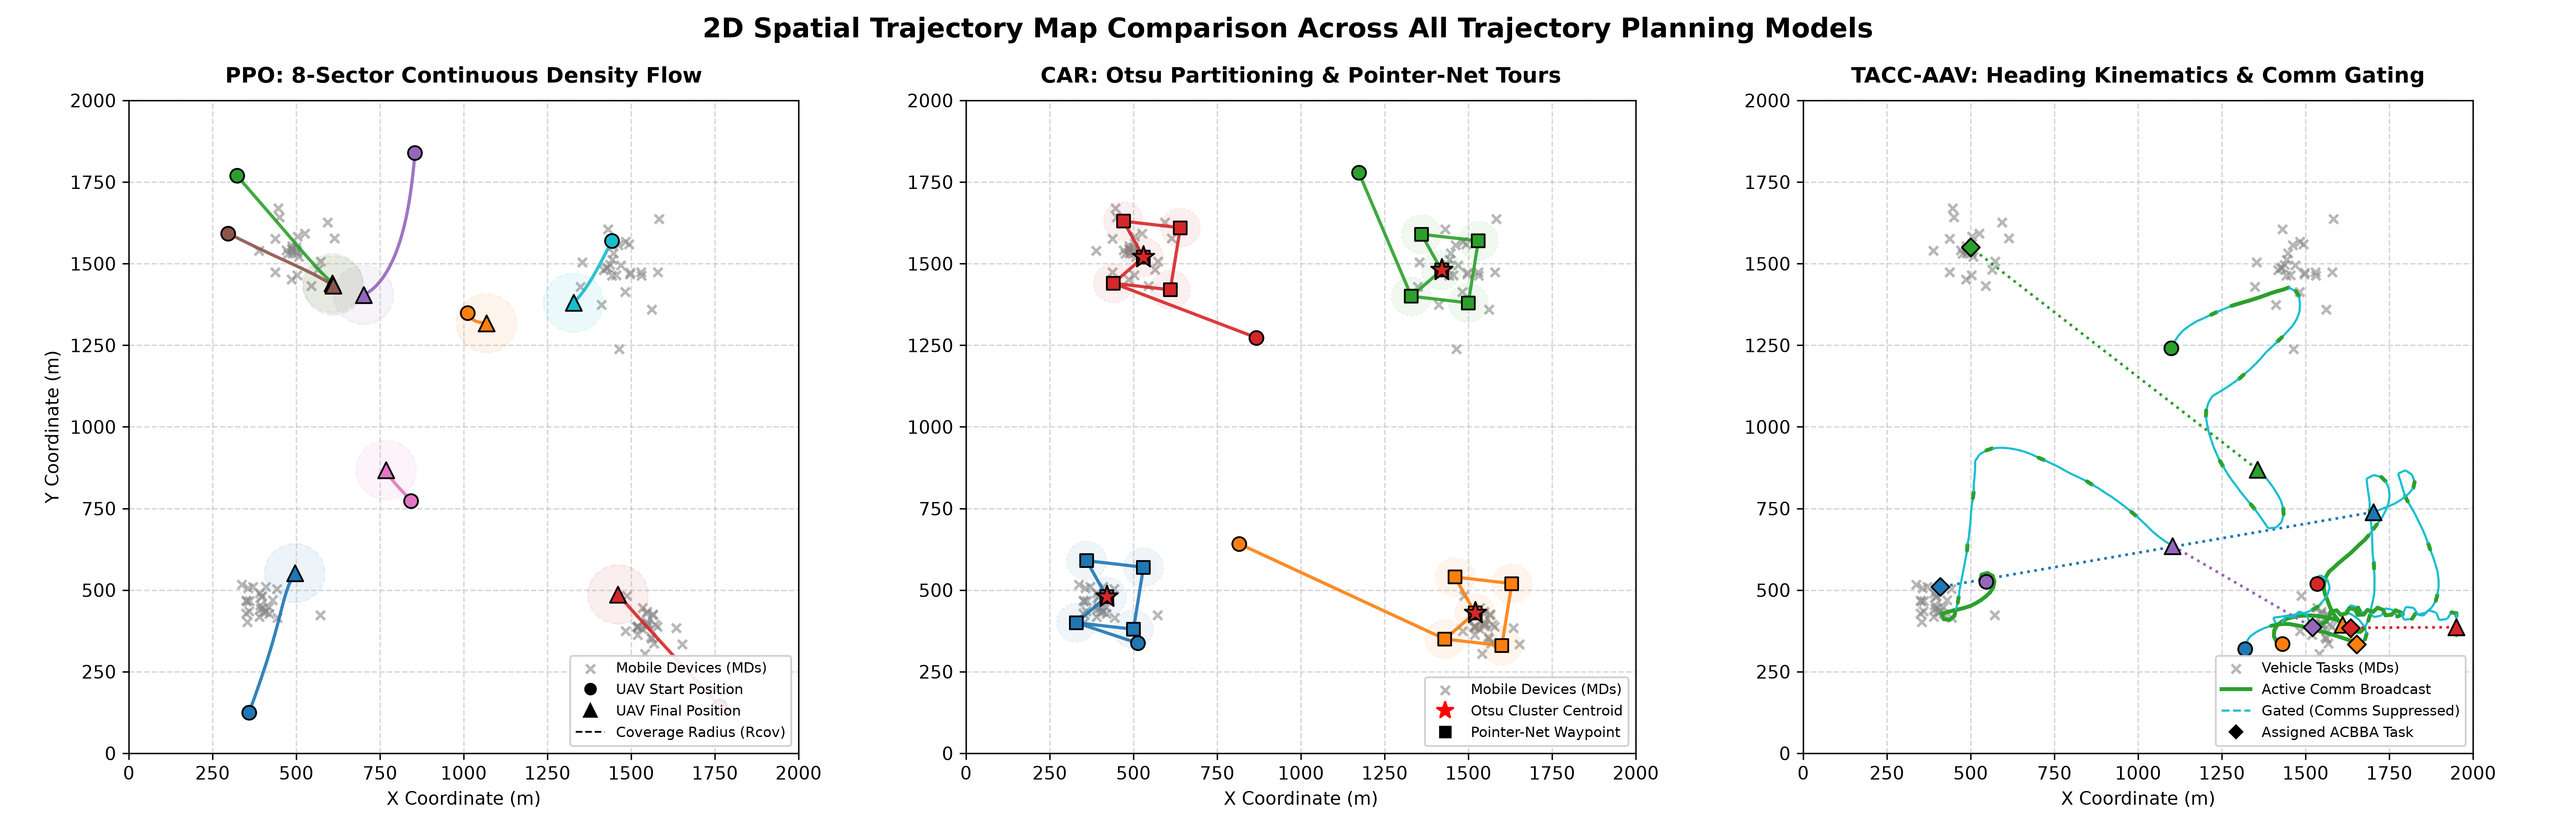
\includegraphics[width=0.92\textwidth]{trajectory_maps_all.png}
    \caption{2D spatial flight trajectories across the $2000\,\text{m} \times 2000\,\text{m}$ simulation field: (a) PPO continuous density flow converging into central MD hot spots; (b) CAR Otsu region partitioning, cluster centroids ($\bigstar$), square waypoints ($\blacksquare$), and Pointer-Net TSP tour routes; (c) TACC-AAV continuous heading kinematics with MOCPO communication gating (solid green = active broadcast, dashed cyan = gated/suppressed broadcast) and ACBBA task bundle links ($\blacklozenge$).}
    \label{fig:trajectory_maps}
\end{figure*}

\textbf{Spatial Trajectory Inferences:}
\begin{itemize}
    \item \textit{PPO Hotspot Convergence and Peripheral Starvation (Fig.~\ref{fig:trajectory_maps}(a)):} Drones guided by local 8-sector density gradients all gravitate toward the same high-density MD clusters. This produces severe multi-drone coverage overlap in the center, while vast peripheral regions remain completely unserved. Once central UAV buffers reach capacity ($C_j = 150$), additional offloading requests are rejected, capping PPO success between $5.61\%$ and $13.81\%$.
    \item \textit{CAR Geometric Partitioning and Patrol Loops (Fig.~\ref{fig:trajectory_maps}(b)):} Otsu thresholding decomposes the theater into four discrete spatial sectors with designated centroids ($\bigstar$). Pointer Networks construct closed TSP loops traversing localized waypoints ($\blacksquare$). By distributing the UAV swarm across all quadrants, CAR eliminates multi-drone crowding, prevents coverage redundancy, and balances task offloading across the entire operational area.
    \item \textit{TACC-AAV Communication Gating and Heading Guidance (Fig.~\ref{fig:trajectory_maps}(c)):} TACC-AAV executes continuous $[v_j, \vartheta_j]$ flight paths conditioned on winning consensus bundles ($\blacklozenge$). The MOCPO gating policy segments paths into active broadcast epochs (solid green) and gated/suppressed epochs (dashed cyan), achieving an exact $50.0\%$ reduction in broadcast packets.
\end{itemize}

\subsection{Inference 3: Temporal Throughput Dynamics}
Fig.~\ref{fig:throughput_time} depicts the epoch-by-epoch throughput ratio (scheduled tasks / generated tasks) over $100$ simulation cycles.

\begin{figure*}[!t]
    \centering
    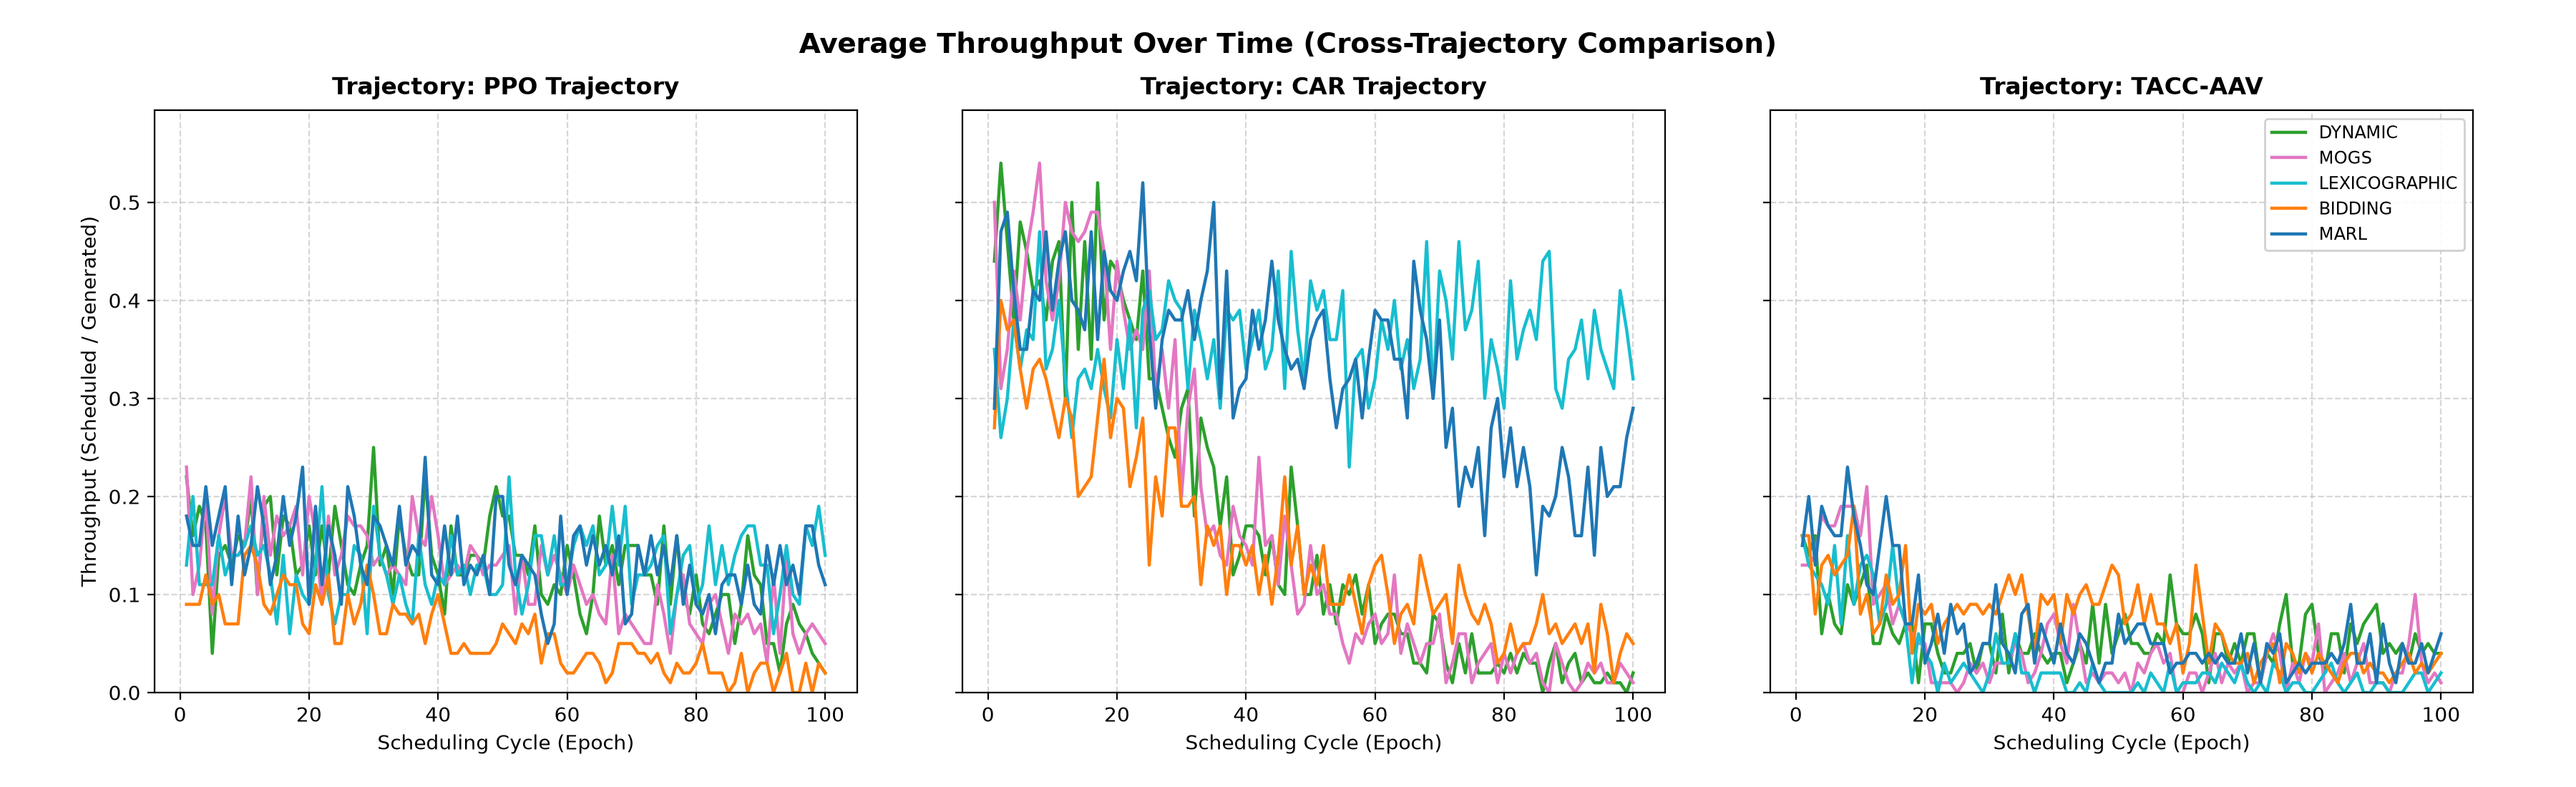
\includegraphics[width=0.92\textwidth]{throughput_comparison.png}
    \caption{Temporal throughput evolution (scheduled tasks / generated tasks) over $100$ cycles across PPO (left), CAR (center), and TACC-AAV (right). CAR sustains significantly higher throughput due to global spatial coverage.}
    \label{fig:throughput_time}
\end{figure*}

\textbf{Temporal Throughput Inferences:}
\begin{itemize}
    \item CAR maintains steady, sustained throughput between $0.30$ and $0.50$ under LEXICOGRAPHIC and MARL across all epochs. Its cyclical waypoint patrol ensures continuous renewal of reachable MD sets.
    \item PPO fluctuates erratically between $0.05$ and $0.25$ because UAVs trapped in central hot spots experience severe buffer saturation and cannot service newly arriving bursts.
    \item TACC-AAV demonstrates controlled throughput ($0.05$--$0.15$), as its dynamic capacity model $N_j(E_j)$ proactively suppresses admissions to conserve flight energy.
\end{itemize}

\subsection{Inference 4: Scheduling Algorithm Runtime and Latency Overhead}
Fig.~\ref{fig:runtime_time} records the execution time per scheduling cycle across all configurations.

\begin{figure*}[!t]
    \centering
    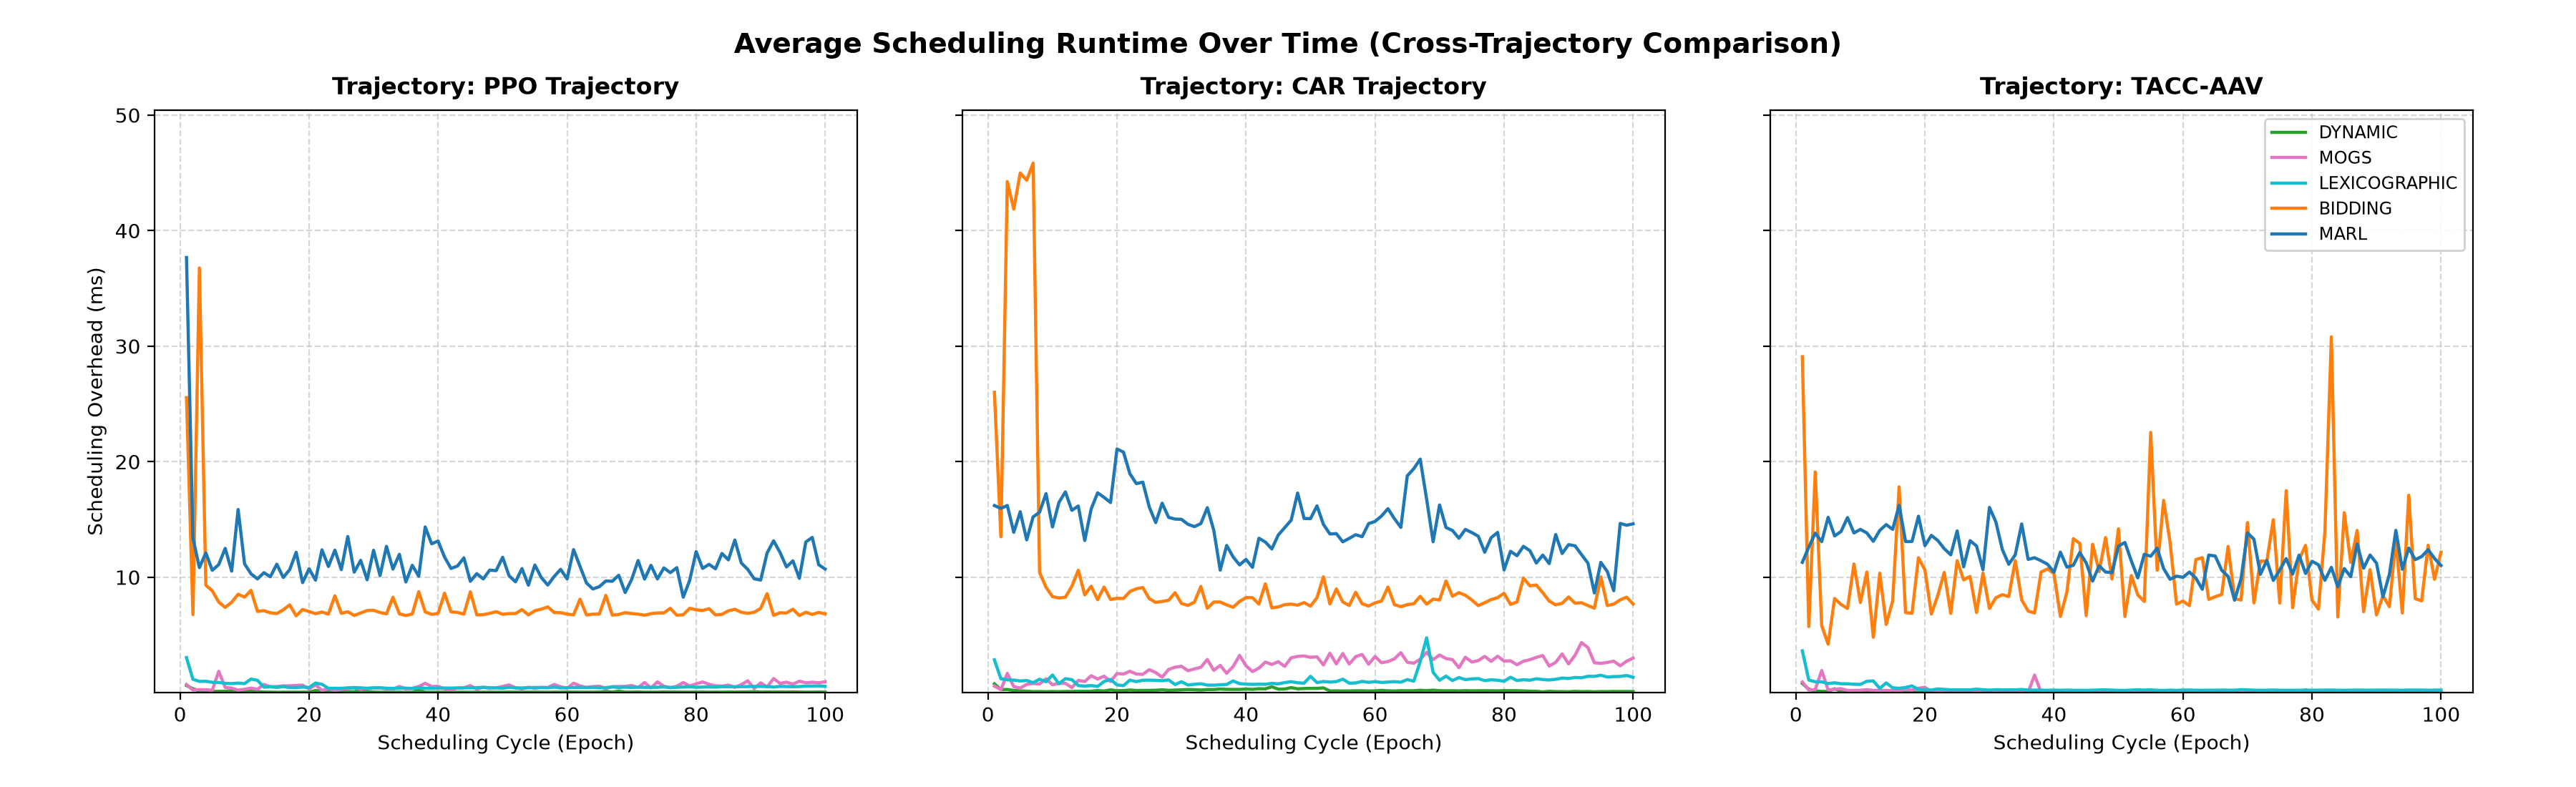
\includegraphics[width=0.92\textwidth]{runtime_comparison.png}
    \caption{Average scheduling runtime overhead (ms) per cycle over $100$ epochs across PPO (left), CAR (center), and TACC-AAV (right). DYNAMIC achieves near-constant sub-millisecond execution, outperforming MARL and iterative auctions by over two orders of magnitude.}
    \label{fig:runtime_time}
\end{figure*}

\textbf{Computational Runtime Inferences:}
\begin{itemize}
    \item DYNAMIC executes in \textbf{0.065--0.205\,ms}, remaining essentially invariant across all trajectory models. By only repairing broken associations ($\mathcal{A}_{\text{broken}}$) and newly arriving tasks via local P2P offloading ($d \le 500\,\text{m}$), DYNAMIC avoids the $O(|\mathcal{K}_t| \cdot |\mathcal{U}|)$ overhead of full graph reconstruction.
    \item MOGS ($0.15$--$2.31\,\text{ms}$) and LEXICOGRAPHIC ($0.35$--$1.10\,\text{ms}$) scale with task batch volume.
    \item BIDDING requires \textbf{7.66--10.36\,ms} due to multi-round communication message passing during auction clearance.
    \item MARL incurs \textbf{11.22--14.41\,ms} per cycle, driven by deep neural network forward passes through RequestNet and ResponseNet, rendering it unsuitable for sub-10ms flight control loops.
\end{itemize}

\subsection{Inference 5: Swarm Workload Balancing (Jain's Fairness Index)}
Fig.~\ref{fig:fairness_time} illustrates the temporal evolution of Jain's Fairness Index:
\begin{equation}
    \mathcal{J} = \frac{\left(\sum_{j=1}^N L_j\right)^2}{N \sum_{j=1}^N L_j^2}, \quad L_j = \frac{|\mathcal{Q}_j|}{C_j}.
\end{equation}

\begin{figure*}[!t]
    \centering
    
\includegraphics[width=0.92\textwidth]{fairness_comparison.png}
    \caption{Swarm workload balancing evaluated via Jain's Fairness Index ($\mathcal{J}$) across $100$ simulation epochs for PPO (left), CAR (center), and TACC-AAV (right). CAR achieves the highest balance ($\mathcal{J} > 0.81$) across all schedulers.}
    \label{fig:fairness_time}
\end{figure*}

\textbf{Fairness Inferences:}
\begin{itemize}
    \item Under CAR, Jain's Index rapidly ascends and stabilizes at $\mathcal{J} > 0.81$ across all schedulers. The four Otsu regions distribute ground workload uniformly across all 30 UAVs.
    \item Under PPO, greedy schedulers assign all tasks to the few drones in the central hotspot, driving their queue utilization $L_j \to 1.0$ while outer drones remain at $L_j \approx 0$, collapsing fairness to $\mathcal{J} \le 0.369$.
    \item DYNAMIC's cooperative P2P offloading redistributes excess tasks from saturated UAVs to nearby peers ($d \le 500\,\text{m}$), boosting PPO fairness to \textbf{0.614} and TACC-AAV fairness to \textbf{0.665}.
\end{itemize}

\subsection{Inference 6: Deadline Slack Margin and Battery-Aware Headroom}
Fig.~\ref{fig:slack_time} plots the average normalized deadline slack margin:
\begin{equation}
    \bar{S} = \frac{1}{|\mathcal{K}_{\text{sched}}|} \sum_{k \in \mathcal{K}} \max\left(0, \; \frac{T_k^{\text{tol}} - (T_{\text{tx}} + T_{\text{proc}} + T_{\text{queue}})}{T_k^{\text{tol}}}\right).
\end{equation}

\begin{figure*}[!t]
    \centering
    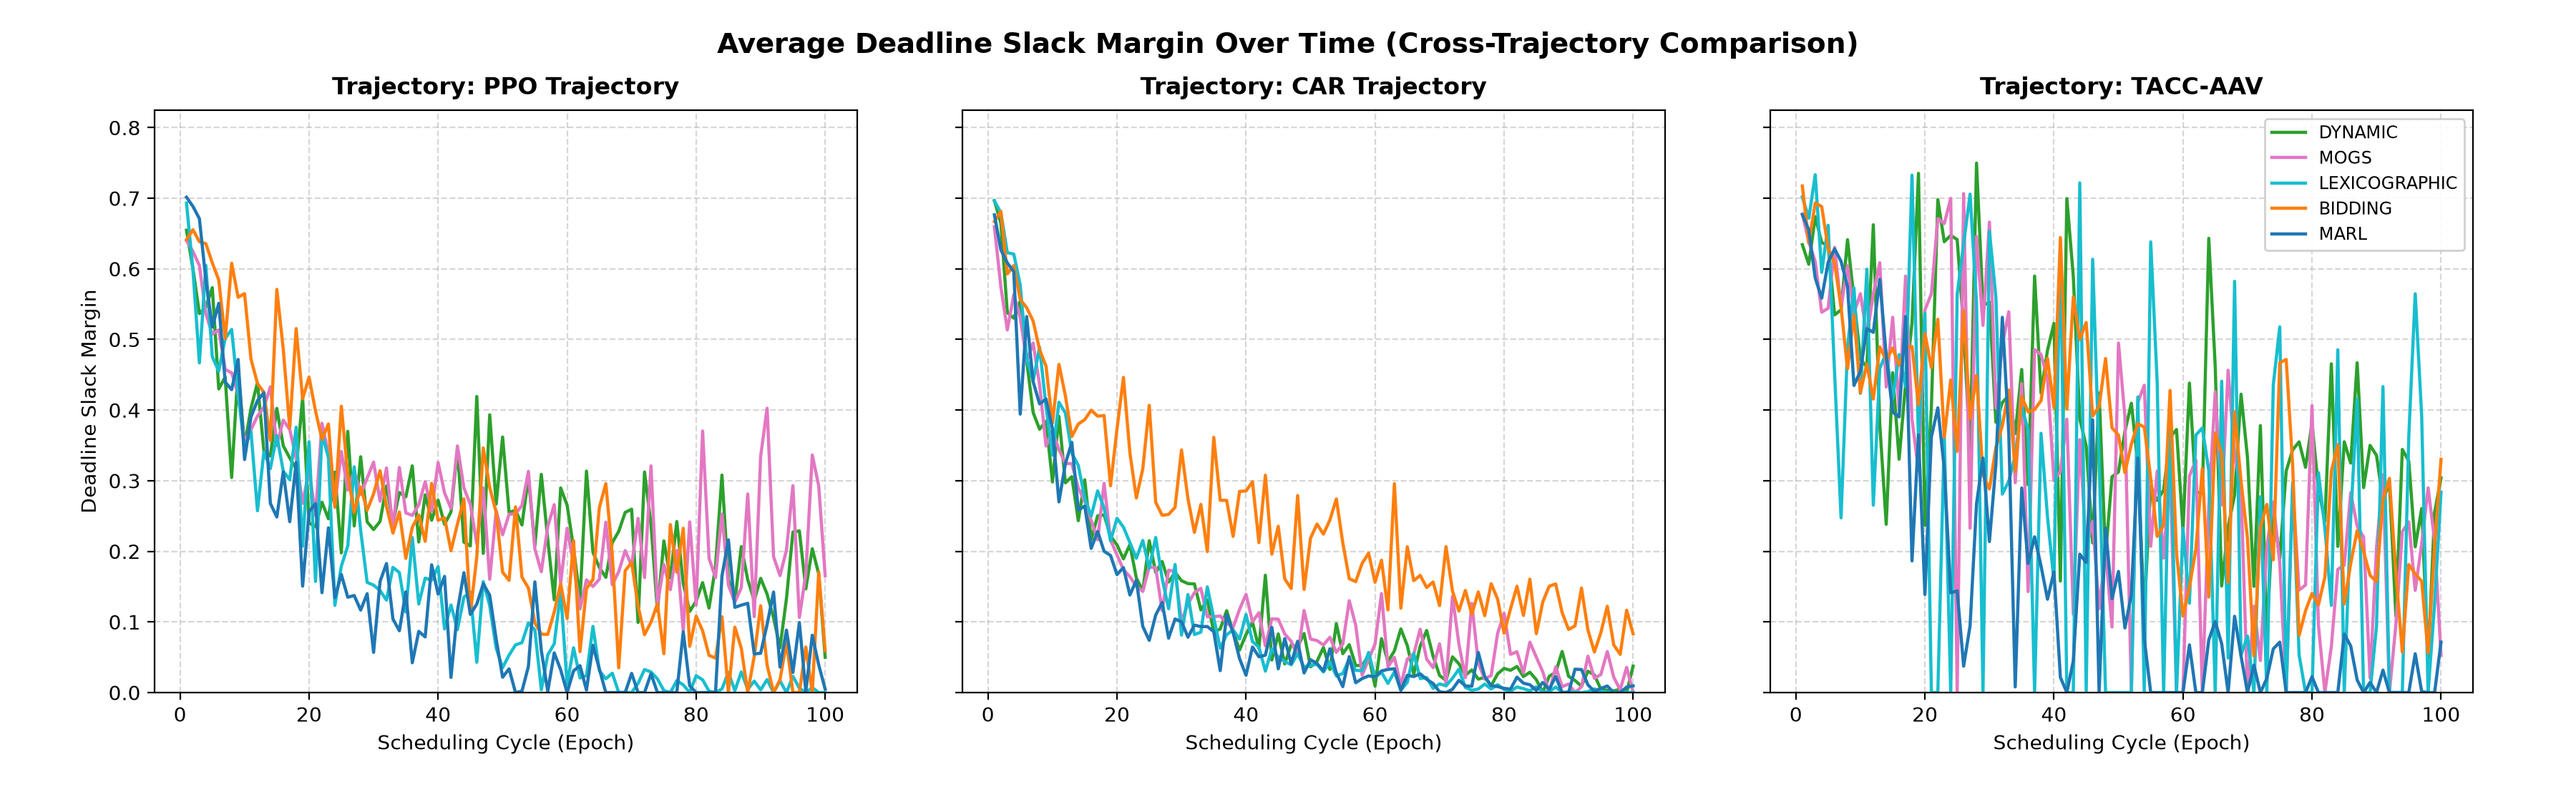
\includegraphics[width=0.92\textwidth]{slack_margin_comparison.png}
    \caption{Average deadline slack margin ($\bar{S}$) over $100$ simulation epochs across PPO (left), CAR (center), and TACC-AAV (right). TACC-AAV maximizes safety slack by coupling dynamic battery headroom with admission gating.}
    \label{fig:slack_time}
\end{figure*}

\textbf{Slack Margin Inferences:}
\begin{itemize}
    \item TACC-AAV achieves the highest slack margin across all configurations, reaching \textbf{0.392} with DYNAMIC and \textbf{0.351} with BIDDING. Its battery-constrained dynamic capacity $N_j(E_j)$ prevents buffer bloat, ensuring minimal queuing delay $T_{\text{queue}}$.
    \item CAR processes high task volumes, causing deeper queue backlogs and lower slack margins ($0.109$--$0.246$).
    \item PPO yields intermediate slack ($0.144$--$0.276$).
\end{itemize}

\subsection{Inference 7: Task Allocation Churn Dynamics}
Fig.~\ref{fig:churn_time} presents the task allocation churn rate, quantifying the frequency of invalidated task-UAV links ($d(i, j) > R_{\text{cov}}$) per epoch caused by aerial mobility.

\begin{figure*}[!t]
    \centering
    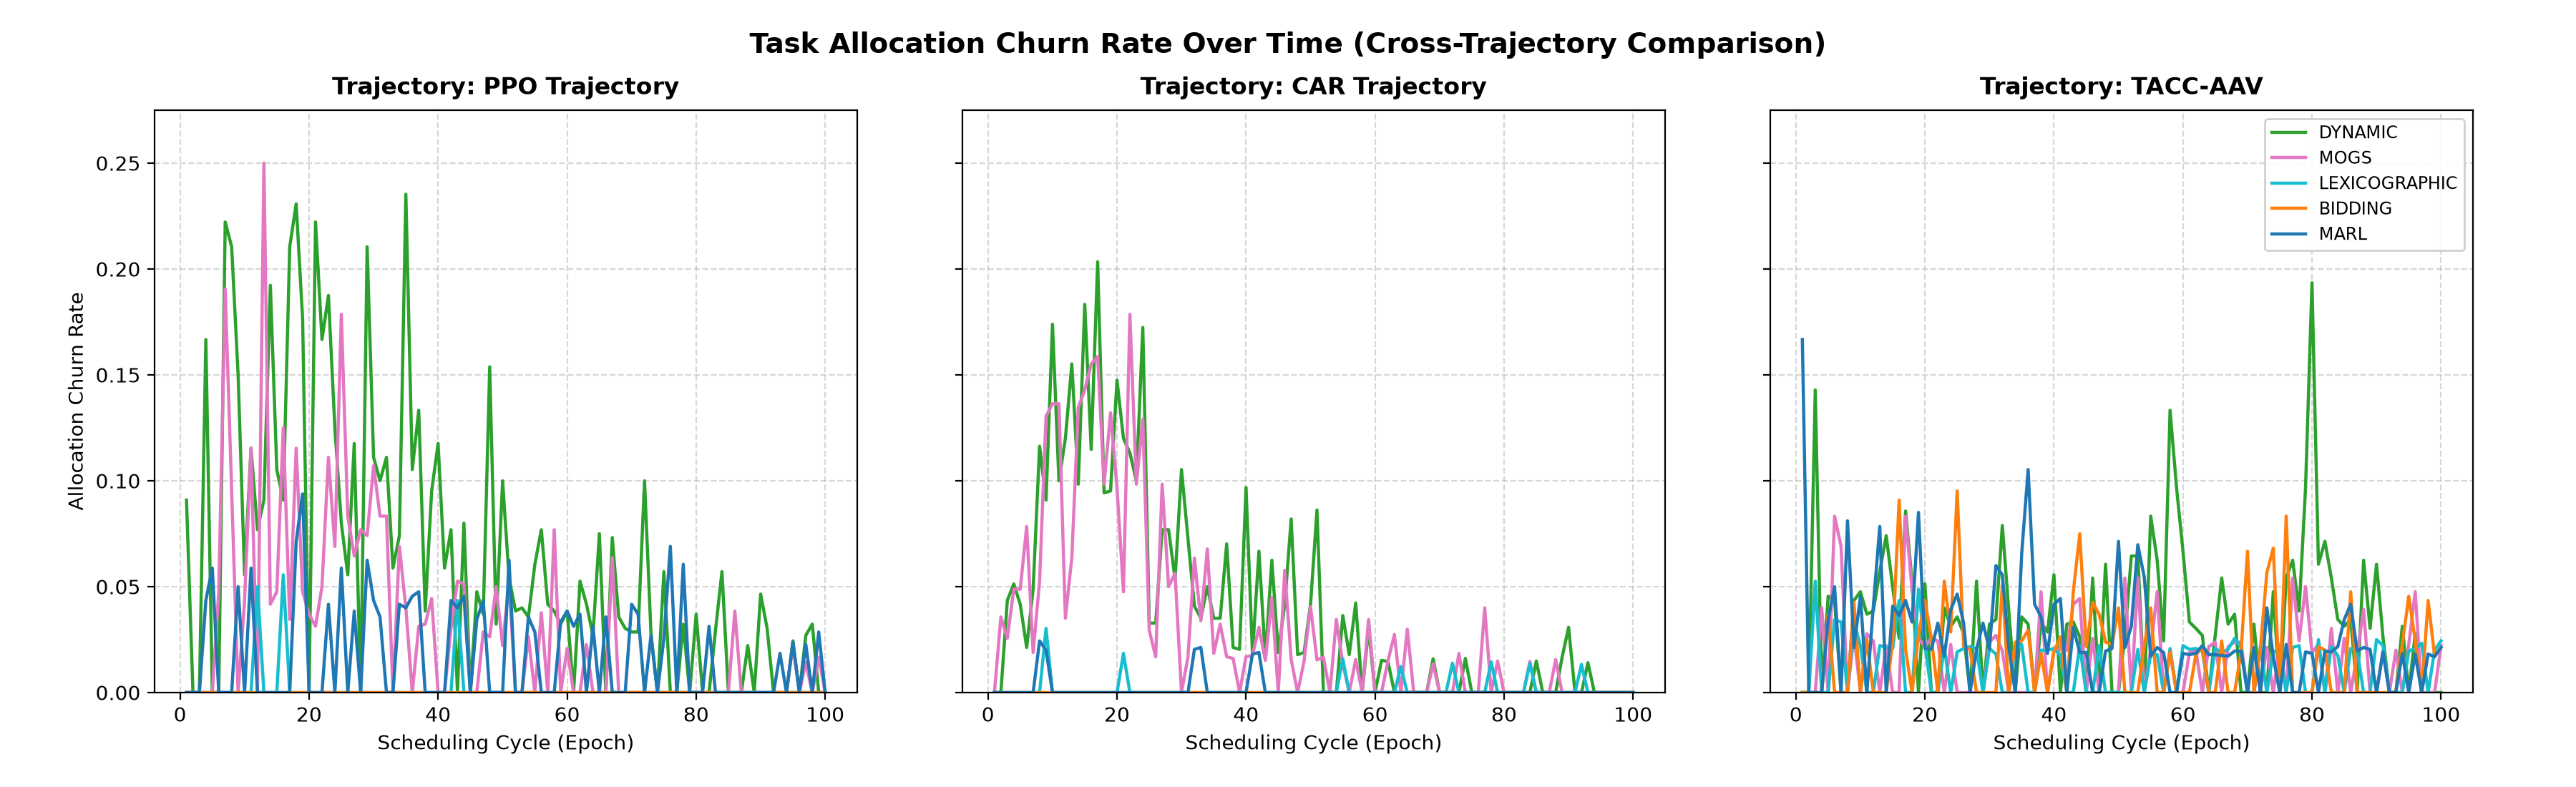
\includegraphics[width=0.92\textwidth]{churn_comparison.png}
    \caption{Task allocation churn rate over $100$ simulation epochs across PPO (left), CAR (center), and TACC-AAV (right). Dynamic matching isolates broken links without causing cascading network churn.}
    \label{fig:churn_time}
\end{figure*}

\textbf{Allocation Churn Inferences:}
\begin{itemize}
    \item Under CAR, high-speed waypoint traversal ($v = 22\,\text{m/s}$) produces consistent link invalidation as drones enter and exit cluster zones.
    \item Baseline matching schedulers (MOGS, LEXICOGRAPHIC, BIDDING, MARL) discard all assignments and recompute the bipartite graph, multiplying communication and computational overhead.
    \item In contrast, DYNAMIC selectively extracts broken links ($|\mathcal{A}_{\text{broken}}| \ll |\mathcal{A}_{t-1}|$) into the repair queue, maintaining allocation stability for unaffected tasks.
\end{itemize}

\subsection{Inference 8: UAV Queue Length Backlog and Buffer Congestion}
Fig.~\ref{fig:queue_time} charts the average unassigned task backlog and buffer occupancy across the UAV fleet over $100$ epochs.

\begin{figure*}[!t]
    \centering
    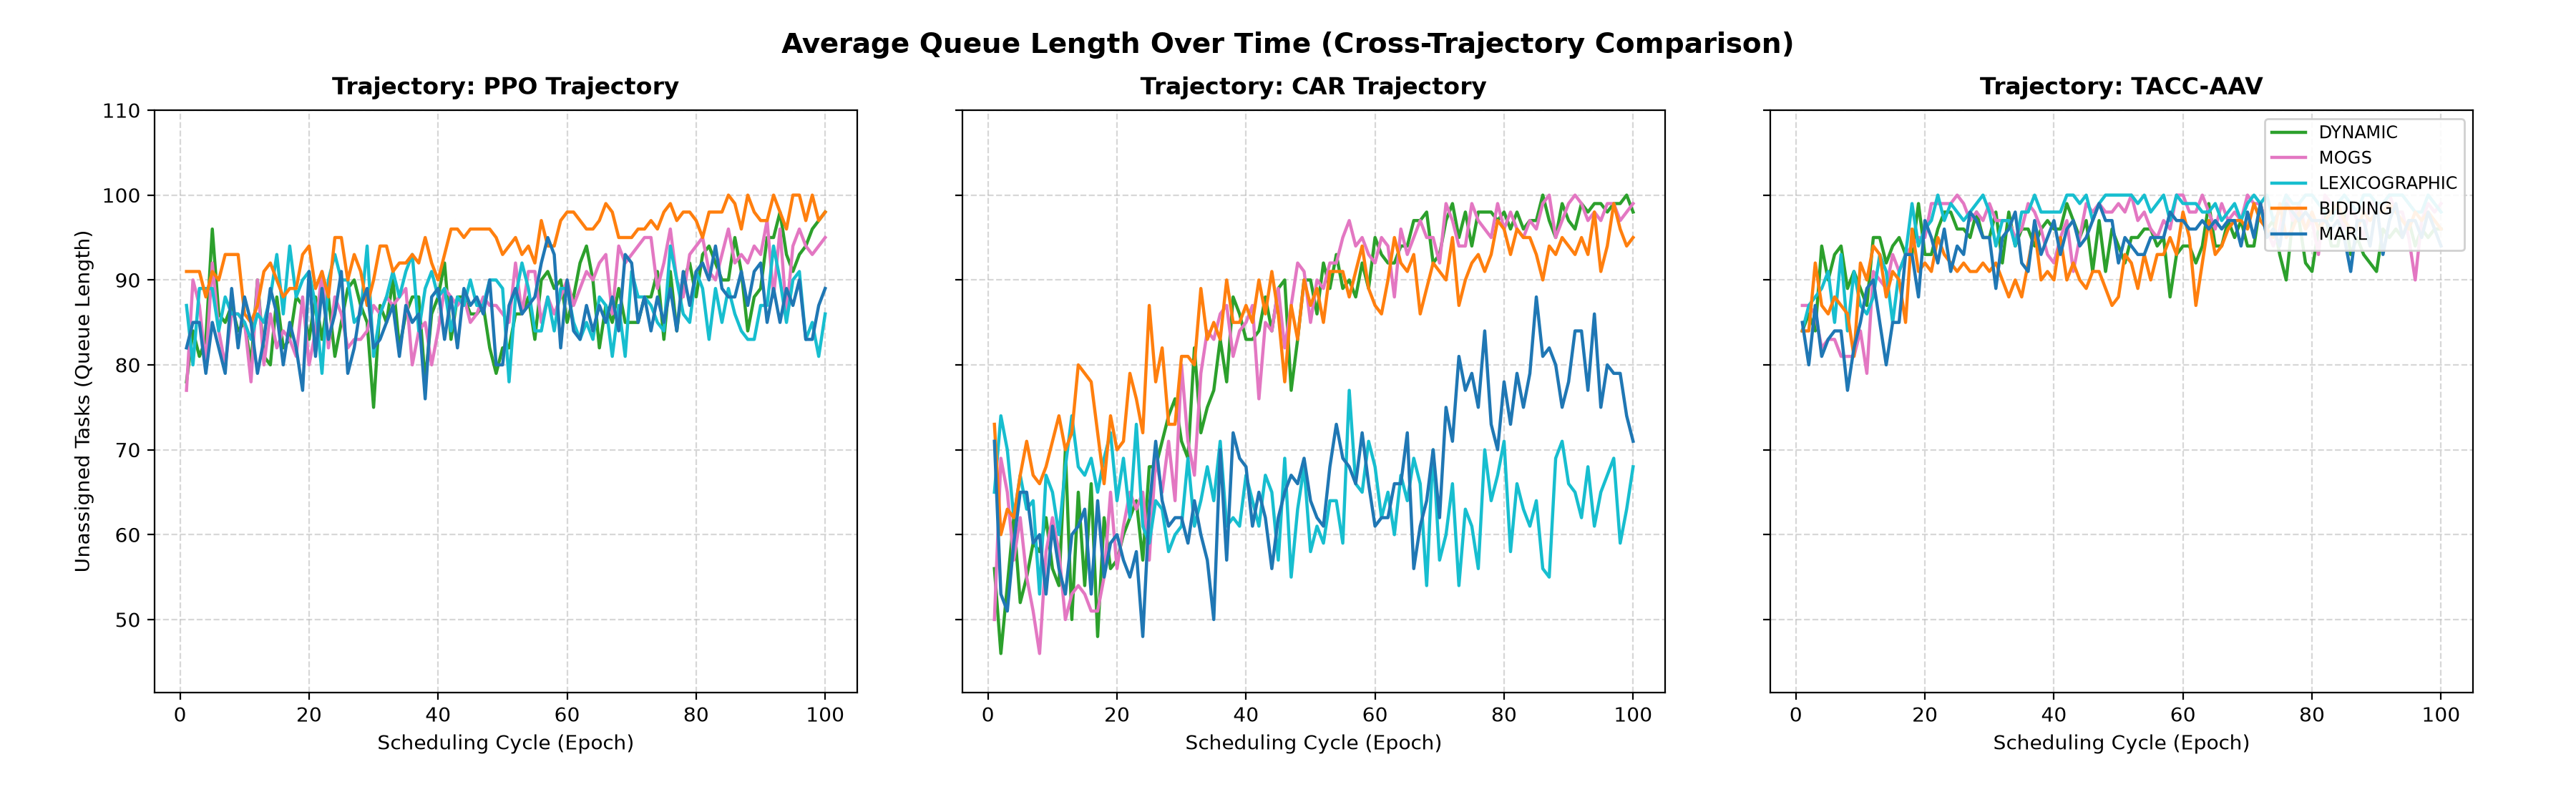
\includegraphics[width=0.92\textwidth]{queue_length_comparison.png}
    \caption{Average queue length backlog over $100$ cycles across PPO (left), CAR (center), and TACC-AAV (right). PPO experiences severe localized buffer overflow, whereas CAR balances queue occupancy across the fleet.}
    \label{fig:queue_time}
\end{figure*}

\textbf{Queue Backlog Inferences:}
\begin{itemize}
    \item Under PPO, central UAVs suffer persistent buffer overflow ($|\mathcal{Q}_j| \to 150$), while peripheral drones have empty queues ($|\mathcal{Q}_j| = 0$).
    \item CAR distributes queue backlogs evenly across all 30 UAVs, ensuring no individual drone becomes an edge computing bottleneck.
    \item TACC-AAV strictly limits queue depth to $N_j(E_j)$, avoiding buffer congestion entirely.
\end{itemize}

\subsection{Inference 9: Fleet Capacity Utilization Dynamics}
Fig.~\ref{fig:cap_util_time} illustrates fleet-wide capacity utilization ($\sum |\mathcal{Q}_j| / \sum C_j$) over time.

\begin{figure*}[!t]
    \centering
    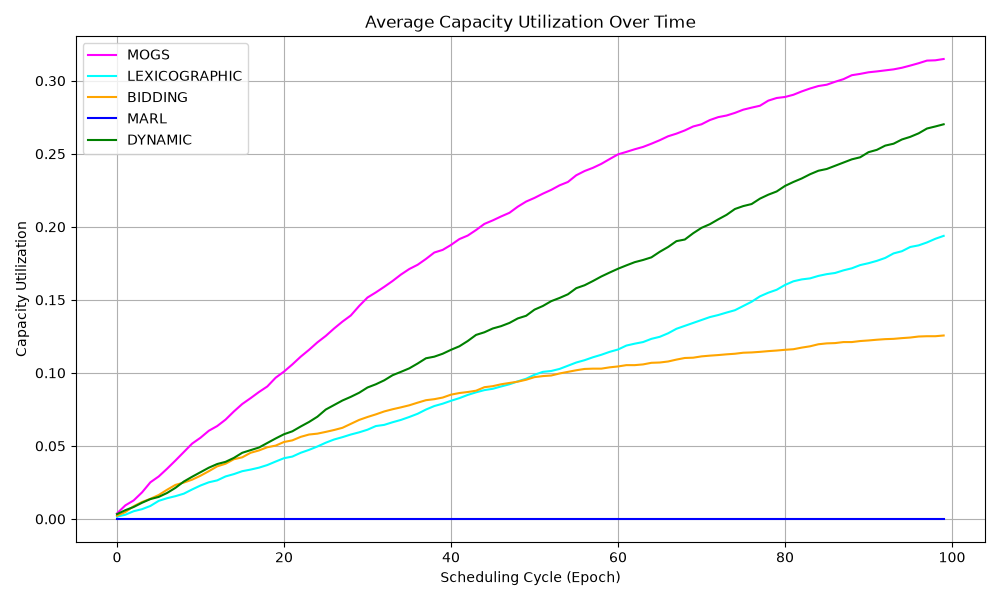
\includegraphics[width=0.92\textwidth]{capacity_utilization_comparison.png}
    \caption{Fleet capacity utilization over $100$ simulation epochs across PPO (left), CAR (center), and TACC-AAV (right). CAR achieves the highest hardware capacity utilization.}
    \label{fig:cap_util_time}
\end{figure*}

\textbf{Capacity Utilization Inferences:}
\begin{itemize}
    \item CAR achieves the highest sustained capacity utilization ($> 60\%$) under LEXICOGRAPHIC and MARL, maximizing compute resource utilization across the aerial fleet.
    \item PPO caps utilization around $25\%$--$35\%$, as idle peripheral drones drag down swarm averages.
    \item TACC-AAV dynamically contracts capacity as battery reserve drops, maintaining conservative utilization ($15\%$--$25\%$) to prevent mid-air battery exhaustion.
\end{itemize}

\end{document}

